% BAC 2022 D - Exercice 2
% Plan complexe - Points A, B, C, D et ensembles E, F

\documentclass[border=5pt]{standalone}
\usepackage{tikz}
\usepackage{amsmath}
\usepackage{amssymb}

\begin{document}

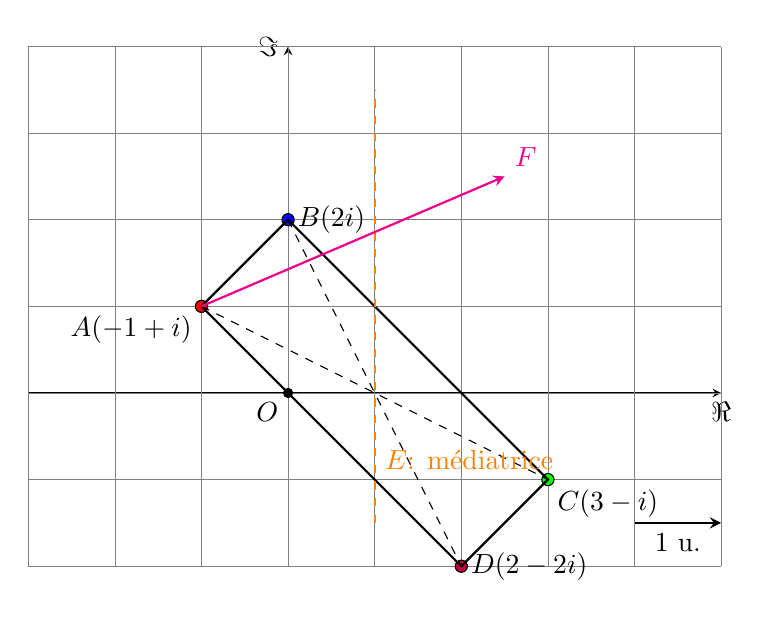
\begin{tikzpicture}[scale=1.1, >=stealth]

% Axes
\draw[->] (-3,0) -- (5,0) node[below] {$\Re$};
\draw[->] (0,-2) -- (0,4) node[left] {$\Im$};

% Grid
\draw[help lines] (-3,-2) grid (5,4);

% Points
% A: z_A = -1 + i
\coordinate (A) at (-1,1);
\draw[fill=red] (A) circle (2pt);

% B: z_B = 2i
\coordinate (B) at (0,2);
\draw[fill=blue] (B) circle (2pt);

% C: z_C = 3 - i
\coordinate (C) at (3,-1);
\draw[fill=green] (C) circle (2pt);

% D: parallélogramme ABCD -> D = A + C - B = (-1+1) + (3-1) - (0+2i) = 2 - 2i
\coordinate (D) at (2,-2);
\draw[fill=purple] (D) circle (2pt);

% Labels
\node[below left] at (A) {$A(-1+i)$};
\node[right] at (B) {$B(2i)$};
\node[below right] at (C) {$C(3-i)$};
\node[right] at (D) {$D(2-2i)$};

% Draw parallelogram
\draw[thick] (A) -- (B) -- (C) -- (D) -- (A);
\draw[dashed] (A) -- (C);
\draw[dashed] (B) -- (D);

% Origin
\draw[fill=black] (0,0) circle (1.5pt) node[below left] {$O$};

% Ensemble E: médiatrice de [M1M2] où M1(3,-1) et M2(-1,1)
% C'est la médiatrice du segment entre C(3,-1) et A(-1,1)
\draw[orange, thick, dashed] (1,-1.5) -- (1,3.5) 
    node[pos=0.1, above right] {$E$: médiatrice};

% Ensemble F: demi-droite issue de A formant angle droit avec AC
% L'angle entre AM et AC est π/2
\draw[magenta, thick, ->] (A) -- (2.5,2.5) node[above right] {$F$};

% Scale
\draw[->, thick] (4,-1.5) -- (5,-1.5) node[midway, below] {1 u.};

\end{tikzpicture}

\end{document}